% % \DocumentMetadata{testphase={phase-III,math,table}}
\documentclass[12pt]{article}
\input{preamble}
\input{config}


\begin{document}
\begin{center}
    \color{BlueViolet}

     \textbf{\newline\newline}
    \vspace{6pt}
    \large
    \textbf{\\HO CHI MINH UNIVERSITY OF SCIENCE}
    

    
    \vspace{6pt}
    \large
    \textbf{\\FACULTY OF INFORMATION TECNOLOGY}

    \vspace{6pt}
    \large
    \textbf{\\DATA VISUALIZATION}
   
\end{center}

\begin{center}
    
\includegraphics[scale=0.25,alt={Logo of HCMUS}]{images/Logo_HCMUS.png}
    \color{BlueViolet}
    
   \large
   \textbf{LAB 1 REPORT} 
    \vspace{25pt}\\

    \color{BlueViolet}
    \textbf{LECTURER:} 
    \color{Black}
    \\ Võ Nhật Tân
    \vspace{15pt}\\


    \color{BlueViolet}
    \textbf{STUDENT (GROUP 2):}
    \color{Black}
    \\ Nguyễn Đỗ Bảo - 23127026
    \\ {Lê Nguyên Thảo - 23127118}
    \\ {Đinh Đại Vũ - 23127144}
    \\ {Vũ Hoàng Minh - 23127427}
    \\ {Nguyễn Thanh Owen - 23127447}
    \vspace{25pt}\\

\end{center}

\begin{tikzpicture}[remember picture,overlay,inner sep=0,outer sep=0]
     \draw[blue!70!black,line width=4pt] ([xshift=-1.5cm,yshift=-2cm]current page.north east) coordinate (A)--([xshift=1.5cm,yshift=-2cm]current page.north west) coordinate(B)--([xshift=1.5cm,yshift=2cm]current page.south west) coordinate (C)--([xshift=-1.5cm,yshift=2cm]current page.south east) coordinate(D)--cycle;

     \draw ([yshift=0.5cm,xshift=-0.5cm]A)-- ([yshift=0.5cm,xshift=0.5cm]B)--
     ([yshift=-0.5cm,xshift=0.5cm]B) --([yshift=-0.5cm,xshift=-0.5cm]B)--([yshift=0.5cm,xshift=-0.5cm]C)--([yshift=0.5cm,xshift=0.5cm]C)--([yshift=-0.5cm,xshift=0.5cm]C)-- ([yshift=-0.5cm,xshift=-0.5cm]D)--([yshift=0.5cm,xshift=-0.5cm]D)--([yshift=0.5cm,xshift=0.5cm]D)--([yshift=-0.5cm,xshift=0.5cm]A)--([yshift=-0.5cm,xshift=-0.5cm]A)--([yshift=0.5cm,xshift=-0.5cm]A);


     \draw ([yshift=-0.3cm,xshift=0.3cm]A)-- ([yshift=-0.3cm,xshift=-0.3cm]B)--
     ([yshift=0.3cm,xshift=-0.3cm]B) --([yshift=0.3cm,xshift=0.3cm]B)--([yshift=-0.3cm,xshift=0.3cm]C)--([yshift=-0.3cm,xshift=-0.3cm]C)--([yshift=0.3cm,xshift=-0.3cm]C)-- ([yshift=0.3cm,xshift=0.3cm]D)--([yshift=-0.3cm,xshift=0.3cm]D)--([yshift=-0.3cm,xshift=-0.3cm]D)--([yshift=0.3cm,xshift=-0.3cm]A)--([yshift=0.3cm,xshift=0.3cm]A)--([yshift=-0.3cm,xshift=0.3cm]A);

\end{tikzpicture}
\newpage
\renewcommand{\contentsname}{\textbf{Contents}}

\tableofcontents

\newpage
\listoffigures
\listoftables

\newpage
\section*{Group Members}

\begin{table}[H]
\centering
\renewcommand{\arraystretch}{1.4}
\begin{tabularx}{\textwidth}{|c|X|c|c|}
\hline
\textbf{No.} & \textbf{Full Name} & \textbf{Student ID} & \textbf{Contribution} \\ \hline
1 & Nguyễn Đỗ Bảo & 23127026 & 20\% \\ \hline
2 & Lê Nguyên Thảo & 23127118 & 20\% \\ \hline
3 & Đinh Đại Vũ & 23127144 & 20\% \\ \hline
4 & Vũ Hoàng Minh & 23127427 & 20\% \\ \hline
5 & Nguyễn Thanh Owen & 23127447 & 20\% \\ \hline
\end{tabularx}
\caption{Group members and stated contribution}
\label{tab:group-members}
\end{table}

\section*{Task Distribution and Completion Status}

\begin{table}[H]
\centering
\small
\renewcommand{\arraystretch}{1.3}
\begin{tabularx}{\textwidth}{|c|X|c|c|c|}
\hline
\textbf{No.} & \textbf{Assigned Work} & \textbf{Responsible} & \textbf{Student ID} & \textbf{Completion} \\ \hline
1 & Data cleaning, preprocessing, and preparation of the final analytical dataset & Nguyễn Thanh Owen & 23127447 & 100\% \\ \hline
2 & Relational database design and Power BI data-model structure & Đinh Đại Vũ & 23127144 & 100\% \\ \hline
3 & Objectives 1.1--1.2: Sales performance by category and time & Đinh Đại Vũ & 23127144 & 100\% \\ \hline
4 & Objectives 2.1--2.2: Finance Structure & Vũ Hoàng Minh & 23127427 & 100\% \\ \hline
5 & Objectives 3.1--3.2: Product influence analysis and dashboard support & Lê Nguyên Thảo & 23127118 & 100\% \\ \hline
6 & Objectives 4.1--4.2: Customer ratings and review-signal analysis & Nguyễn Thanh Owen & 23127447 & 100\% \\ \hline
7 & Objectives 5.1--5.2: Machine learning support and model interpretation & Nguyễn Đỗ Bảo & 23127026 & 100\% \\ \hline
8 & Power BI dashboard design, layout, and visual organization & Lê Nguyên Thảo & 23127118 & 100\% \\ \hline
9 & Report writing, editing, and final content review & Vũ Hoàng Minh & 23127427 & 100\% \\ \hline
10 & Report writing, editing, and final content review & Nguyễn Đỗ Bảo & 23127026 & 100\% \\ \hline
\end{tabularx}
\caption{Task allocation used in this report}
\label{tab:task-distribution}
\end{table}


\newpage
\section{Introduction to the Analytical Problems}
\subsection{Domain Situation}
\subsection{Analytical Objectives}
    \subsubsection{Sales Performance by Category and Time}
    \begin{itemize}
        \item \textbf{Objective 1}: Measure how total revenue is distributed across Nike product categories from February 20, 2026 to March 20, 2026 in order to identify the highest-contributing categories and assess whether sales performance is concentrated in a small number of categories.
        \begin{itemize}
            \item \textbf{Specific}: Category-level revenue contribution analysis aligned with the KPI cards and the \texttt{Total Revenue by Category name} bar chart.
            \item \textbf{Measurable}: Uses \texttt{Total Daily Revenue}, \texttt{Average Revenue per Day}, \texttt{Revenue Difference}, and \texttt{Total Revenue by category\_name}.
            \item \textbf{Achievable}: All required revenue measures and category fields are available in the prepared sales dataset and current dashboard design.
            \item \textbf{Relevant}: Directly supports the group's analytical problem by showing how product category influences sales performance.
            \item \textbf{Time-bound}: Evaluated within the analytical window from 20-02-2026 to 20-03-2026.
        \end{itemize}
    \end{itemize}

    \begin{itemize}
        \item \textbf{Objective 2}: Compare the most volatile and most stable Nike product categories over February 20, 2026 to March 20, 2026 in order to determine which categories show consistent sales performance over time and which categories experience stronger revenue fluctuations.
        \begin{itemize}
            \item \textbf{Specific}: Time-based category stability analysis using the \texttt{Top 3 Most Volatile Categories} and \texttt{Top 3 Most Stable Categories} visuals.
            \item \textbf{Measurable}: Uses \texttt{Category Revenue CV} to compare the relative revenue fluctuation of categories across the analytical period.
            \item \textbf{Achievable}: The required category-level revenue variation metric is available in the prepared model outputs and dashboard visuals.
            \item \textbf{Relevant}: Directly supports the analytical problem by showing how category-level sales performance changes over time, not just in total size.
            \item \textbf{Time-bound}: Evaluated within the same analytical window from 20-02-2026 to 20-03-2026.
        \end{itemize}
    \end{itemize}

    \subsubsection{Pricing and Discount Strategy}
    \begin{itemize}
        \item \textbf{Objective 1}: Measure revenue-share and unit-share differences across predefined Price Band groups from February 20, 2026 to March 20, 2026 in order to identify the dominant price band in the current dashboard design.
        \begin{itemize}
            \item \textbf{Specific}: Price-band contribution analysis aligned with the \texttt{Price distribution} visual.
            \item \textbf{Measurable}: Uses share of \texttt{daily\_revenue}, share of \texttt{daily\_units\_sold}, and \texttt{average selling\_price} by Price Band.
            \item \textbf{Achievable}: \texttt{selling\_price} and sales variables are available in the prepared snapshot dataset.
            \item \textbf{Relevant}: Directly supports interpretation of the KPI cards and pie-chart structure on the dashboard.
            \item \textbf{Time-bound}: Evaluated within the analytical window from 20-02-2026 to 20-03-2026.
        \end{itemize}
    \end{itemize}

    \begin{itemize}
        \item \textbf{Objective 2}: Build a chart-based comparison (line/column with slicers) of KPI changes under date and category filters from February 20, 2026 to March 20, 2026 in order to determine whether sales performance is broad-based or concentrated by segment.
        \begin{itemize}
            \item \textbf{Specific}: Chart-based sensitivity analysis of \texttt{daily\_revenue}, \texttt{daily\_units\_sold}, and \texttt{Average Selling Price} under slicer conditions.
            \item \textbf{Measurable}: Uses KPI percentage change shown on the chart across selected date/category states and compares resulting segment composition.
            \item \textbf{Achievable}: The required KPIs, segment dimensions, and filters are available in the current dashboard and source tables.
            \item \textbf{Relevant}: Matches the interactive dashboard workflow and provides visual evidence for report/viva interpretation.
            \item \textbf{Time-bound}: Limited to the same analytical period from 20-02-2026 to 20-03-2026.
        \end{itemize}
    \end{itemize}

    \subsection{Product Influence Analysis}
    \begin{itemize}
        \item \textbf{Objective 1}: Identify the top products and categories driving daily unit sales from February 20, 2026 to March 20, 2026 using the current Top products visual and dashboard filters.
        \begin{itemize}
            \item \textbf{Specific}: Product-level and category-level contribution analysis focused on unit performance.
            \item \textbf{Measurable}: Uses \texttt{daily\_units\_sold} ranking, top-product share of total units sold, and category composition of top products.
            \item \textbf{Achievable}: \texttt{Product name}, \texttt{category}, and \texttt{daily unit} fields are available in the current dashboard model.
            \item \textbf{Relevant}: Directly supports the page purpose of understanding product influence on sales outcomes.
            \item \textbf{Time-bound}: Evaluated within the analysis window from 20-02-2026 to 20-03-2026.
        \end{itemize}
    \end{itemize}

    \begin{itemize}
        \item \textbf{Objective 2}: Analyze time-based spikes and concentration risk among top products from February 20, 2026 to March 20, 2026 by combining trend visuals with date/category slicers.
        \begin{itemize}
            \item \textbf{Specific}: Temporal sensitivity analysis of top-product unit performance under interactive filters.
            \item \textbf{Measurable}: Uses peak \texttt{daily\_units\_sold} values by date, spike frequency of top products, and concentration ratio of top products versus total units sold.
            \item \textbf{Achievable}: \texttt{Date}, \texttt{product}, \texttt{category}, and unit metrics are available in the current dashboard visuals.
            \item \textbf{Relevant}: Explains whether page-level performance is broad-based or overly dependent on a small number of products.
            \item \textbf{Time-bound}: Limited to the same analytical period from 20-02-2026 to 20-03-2026.
        \end{itemize}
    \end{itemize}

    \subsubsection{Customer Ratings and Review Signals}
    \begin{itemize}
        \item \textbf{Objective 1}: Use the line chart of review count by year to examine how customer review activity changes across 2024, 2025, and 2026, in order to identify whether engagement with Nike products on Lazada is increasing, decreasing, or remaining stable over time.
        \begin{itemize}
            \item \textbf{Specific}: Year-based review activity analysis using \texttt{reviews\_count} across the three observed periods.
            \item \textbf{Measurable}: Uses the trend and year-to-year differences in \texttt{reviews\_count} from 2024 to 2026.
            \item \textbf{Achievable}: The required review \texttt{date} and \texttt{review count} fields are available in the prepared review dataset and dashboard design.
            \item \textbf{Relevant}: Supports the analytical problem by showing how customer review behavior evolves over time, which may relate to product visibility and sales performance.
            \item \textbf{Time-bound}: Evaluated across the yearly periods 2024, 2025, and 2026.
        \end{itemize}
    \end{itemize}

    \begin{itemize}
        \item \textbf{Objective 2}: Use the bar chart of ratings by year to compare customer evaluation levels across 2024, 2025, and 2026, in order to determine whether Nike product ratings remain consistent or show meaningful changes over time.
        \begin{itemize}
            \item \textbf{Specific}: Year-based rating comparison using the average rating level for each year.
            \item \textbf{Measurable}: Uses differences in \texttt{rating} or \texttt{average\_rating} across 2024, 2025, and 2026.
            \item \textbf{Achievable}: The required \texttt{rating} and \texttt{review-date} fields are available in the prepared review dataset and dashboard visuals.
            \item \textbf{Relevant}: Supports the analytical problem by showing whether customer satisfaction changes over time and how review behavior may align with perceived product quality.
            \item \textbf{Time-bound}: Evaluated across the yearly periods 2024, 2025, and 2026.
        \end{itemize}
    \end{itemize}

    \subsubsection{Segment Clustering and Revenue Contribution}
    \begin{itemize}
        \item \textbf{Objective 1: Clustering Quality and Segment Identification} - Use the silhouette score comparison bar chart and the cluster scatter chart to evaluate the clustering solution and identify distinct Nike product groups from February 20, 2026 to March 20, 2026, in order to show that the dataset can be meaningfully segmented into different sales-performance patterns.
        \begin{itemize}
            \item \textbf{Specific}: Compare clustering quality across candidate cluster settings using \texttt{silhouette\_score}, then visualize product distribution by \texttt{segment\_id} on the scatter chart.
            \item \textbf{Measurable}: Uses differences in \texttt{silhouette\_score} across cluster options and visible separation of products by \texttt{segment\_id} on the scatter plot.
            \item \textbf{Achievable}: All required fields are available in \texttt{segmentation\_metrics.csv} and \texttt{product\_segments.csv}.
            \item \textbf{Relevant}: Supports the analytical problem by showing that products can be grouped into meaningful clusters before interpreting sales behavior.
            \item \textbf{Time-bound}: Evaluated within the analysis window from 20-02-2026 to 20-03-2026.
        \end{itemize}
    \end{itemize}

    \begin{itemize}
        \item \textbf{Objective 2: Cluster Revenue Contribution Interpretation} - Use the cluster scatter chart together with the pie chart of revenue contribution by cluster to interpret how each product segment contributes to overall Nike sales performance from February 20, 2026 to March 20, 2026, in order to explain which clusters dominate total revenue and which clusters represent smaller but distinct performance groups.
        \begin{itemize}
            \item \textbf{Specific}: Compare revenue contribution across \texttt{segment\_id} and relate each cluster's share of revenue to its position in the cluster scatter chart.
            \item \textbf{Measurable}: Uses \% revenue contribution by cluster, cluster membership on the scatter chart, and differences in \texttt{avg\_daily\_revenue} or \texttt{avg\_total\_period\_revenue}.
            \item \textbf{Achievable}: The required fields are available from \texttt{product\_segments.csv} and \texttt{segment\_profiles.csv}.
            \item \textbf{Relevant}: Directly supports the analytical problem by linking clustered product characteristics to overall sales performance contribution.
            \item \textbf{Time-bound}: Limited to the same analytical period from 20-02-2026 to 20-03-2026.
        \end{itemize}
    \end{itemize}

\newpage
\section{Data Collection, Construction, and Preprocessing}
    \subsection{Product Collection}
    \textbf{Note}: The extraction procedures described in this section were programmatically implemented and executed via the \textbf{\textit{products.py}} script.
        \subsubsection{Objectives and Approach}
        \begin{itemize}
            \item \textbf{Objective}: To systematically collect all product metadata from a specific flagship store on an e-commerce platform (e.g., Lazada). The target data fields include product name, selling price, quantity sold, rating score, and inventory status.
            \item \textbf{Approach}: The system utilizes a Hybrid Web Scraping methodology. This approach combines browser automation (via Selenium) to bypass initial security mechanisms (like Captchas) with direct HTTP requests to optimize data extraction speed and efficiency by querying hidden internal APIs.
        \end{itemize}

        \subsubsection{Detailed Execution Steps}
        \begin{itemize}
            \item \textbf{Step 1: Session Initialization \& Authentication}
            \begin{itemize}
                \item The system initializes a automated browser instance (Google Chrome) using \textbf{Selenium} and \textbf{WebDriverManager}.
                \item It navigates to the target store's homepage. At this point, the execution thread is intentionally paused to allow for manual human intervention. This is necessary to solve complex Captchas or perform account authentication if required by the platform.
                \item Upon successful manual authentication, the system extracts the session \textbf{Cookies} and the browser's \textbf{User-Agent} string.
                \item The automated browser is then terminated to free up system memory, and the process transitions to a lightweight HTTP request mode.
            \end{itemize}

            \item \textbf{Step 2: Category Discovery (Structure Extraction)}
            \begin{itemize}
                \item Utilizing the extracted Cookies and User-Agent, the system simulates an asynchronous HTTP request (AJAX/XMLHttpRequest) directed at the platform's filter API.
                \item The server responds with a JSON payload containing the complete categorical architecture of the store.
                \item The system parses this JSON to isolate the list of product categories and their corresponding internal identifier codes (values), which serve as inputs for the next phase.
            \end{itemize}

            \item \textbf{Step 3: Data Extraction}
            \begin{itemize}
                \item \textbf{Automated Pagination}: The system iterates through each discovered category. Within a category, a while loop is employed to navigate through sequential product pages (page 1, page 2, etc.) by dynamically modifying the page parameter in the API URL.
                \item \textbf{Data Parsing}: For each queried page, the system receives a JSON array of products. The parser extracts core variables: \textit{Item ID}, \textit{Product Name}, \textit{Selling Price}, \textit{Original Price}, \textit{Rating Score}, \textit{Review Count}, \textit{Warehouse Location}, \textit{Stock Status}, \textit{Brand Name}, and \textit{the Product URL}.

                \item \textbf{Data Cleaning}: Unstandardized data formats are processed immediately. For instance, text strings representing sales volume (e.g., "1.5k đã bán") are converted into standard integer formats (1500) using regular expressions to facilitate downstream quantitative analysis.

                \item \textbf{Anti-bot Evasion Mechanism}: The script implements randomized delays (time.sleep between 2 to 3 seconds) between page requests. This simulates organic human browsing behavior, thereby minimizing the risk of IP blocking or rate-limiting by the platform's anti-scraping firewalls

                \item The pagination loop terminates when the API returns an empty product list, indicating the end of the category.
            \end{itemize}

            \item \textbf{Step 4: Data Organization and Storage}
            \begin{itemize}
                \item The system dynamically generates a hierarchical directory structure based on the current execution date (data/MM-DD-YYYY).
                \item The data is simultaneously exported into two formats:
                \begin{itemize}
                    \item \textbf{CSV File} (products.csv): Intended for end-users to easily read, filter, and visualize the data using spreadsheet software like Microsoft Excel.
                    \item \textbf{JSON File} (products.json): Preserves the raw structured format, acting as the requisite input file for the subsequent phase of the project (Review Collection Process).
                \end{itemize}
            \end{itemize}
        \end{itemize}

    \subsection{Review Collection}
    \textbf{Note}: The extraction procedures described in this section were programmatically implemented and executed via the \textbf{\textit{reviews.py}} script.
        \subsubsection{Objectives and Approach}
        \begin{itemize}
            \item \textbf{Objective}: To systematically extract comprehensive customer feedback, including text reviews, star ratings, and timestamps, for all previously identified products to facilitate product quality analysis.
            \item {Approach}: The system employs an API reverse-engineering technique targeting the platform's MTOP architecture. This methodology relies on dynamic cryptographic token generation (MD5 signing), coupled with a local checkpoint system and automated Captcha handling via Selenium, ensuring continuous and resilient data extraction.
        \end{itemize}

        \subsection{Detailed Execution Steps}
        \begin{itemize}
            \item \textbf{Step 1: Data Initialization and Checkpointing}
            \begin{itemize}
                \item The system parses the \textit{products.json} file generated in the first phase. To optimize execution time and prevent data duplication in the event of network interruptions, it implements a checkpoint mechanism. It compares the input list against the existing \textit{reviews.json} output file to bypass products that have already been successfully scraped.
            \end{itemize}

            \item \textbf{Step 2: Session Initialization and Token Extraction} 
            \begin{itemize}
                \item A Selenium-driven browser is temporarily launched to navigate to a sample product page. The primary purpose of this action is not to parse the HTML document, but to force the e-commerce server to issue a specific session cookie (\_m\_h5\_tk). This cookie acts as a fundamental security token for authenticating subsequent API requests.
            \end{itemize}

            \item \textbf{Step 3: Cryptographic Signature Generation (MD5)}
            \begin{itemize}
                \item To bypass the platform's API security layer, the system dynamically generates an MD5 hash signature for every request. This signature is constructed by concatenating the extracted security token, the current Unix timestamp, a hardcoded AppKey, and the stringified JSON payload containing the request parameters (e.g., \textbf{itemId} and \textbf{pageNo}).
            \end{itemize}

            \item \textbf{Step 4: Data Extraction and Pagination}
            \begin{itemize}
                \item The script iterates through the remaining product IDs. For each product, it sends signed HTTP GET requests to the review API, automatically paginating through the results (handling up to a predefined limit, such as 50 pages or 1000 reviews per item). The parser extracts core variables from the server's JSON response, specifically the \textit{Product ID}, \textit{Star Rating}, \textit{Review Content}, and \textit{Timestamp}.
            \end{itemize}

            \item \textbf{Step 5: Real-time Persistence and Anti-bot Evasion:}
            \begin{itemize}
                \item To mitigate the risk of data loss, the extracted reviews are appended to the local storage immediately after processing each individual product. Furthermore, if the system encounters a rate-limit or an anti-bot block signal (e.g., returning a FAIL\_SYS\_USER\_VALIDATE error), it halts the loop, automatically reopens the Selenium browser to allow for manual Captcha resolution, regenerates the security tokens, and seamlessly resumes the crawling process from the exact point of interruption.
            \end{itemize}
        \end{itemize}
    
    \subsection{Data Preparation}
    This section outlines the data cleaning, and feature engineering procedures. Please note that the subsequent Exploratory Data Analysis (EDA) and its visualizations are documented in a separate supplementary file (\textit{\textbf{eda.ipynb}})
        \subsubsection{Product Metadata Dataset}
        This dataset captures the overarching catalog details and aggregate performance metrics for each item in the flagship store. Each row represents a unique product.
        \begin{itemize}
            \item \textbf{id (Primary Key)}: The unique alphanumeric identifier assigned to the product by the e-commerce platform.
            \item \textbf{ten\_san\_pham (Product Name)}: The full, descriptive title of the item as displayed on the storefront.
            \item \textbf{danh\_muc (Category)}: The specific classification of the product (e.g., specific shoe lines, apparel categories) scraped directly from the store's filter menu.
            \item \textbf{gia\_ban (Selling Price)}: The current transactional price of the item, reflecting any active discounts.
            \item \textbf{gia\_goc (Original Price)}: The baseline retail price of the item before any promotional deductions.
            \item \textbf{so\_luong\_da\_ban (Sales Volume)}: A quantitative integer representing the historical number of units sold.
            \item \textbf{diem\_danh\_gia (Rating Score)}: The aggregated average star rating for the product, ranging from 1.0 to 5.0.
            \item \textbf{so\_luot\_nhan\_xet (Review Count)}: The total number of customer ratings the product has accumulated.
            \item \textbf{dia\_diem\_kho (Warehouse Location)}: The geographical origin or fulfillment center location for the item.
            \item \textbf{ton\_kho (Inventory Status)}: A categorical indicator specifying whether the item is currently "Còn hàng" (In-Stock) or "Hết hàng" (Out-of-Stock).
            \item \textbf{thuong\_hieu (Brand)}: The brand name associated with the item .
            \item \textbf{link\_san\_pham (Product URL)}: The fully qualified hyperlink to the product's detail page.
        \end{itemize}

        \subsubsection{Data Cleaning and Standardization For Product Dataset}
        \begin{itemize}
            \item \textbf{Missing Value Imputation}: Null review counts (so\_luot\_nhan\_xet) were filled with 0, while missing rating scores (diem\_danh\_gia) were kept as NaN to prevent skewing the mean during statistical analysis.
            
            \item \textbf{Data Type Casting}: Converted financial and metric columns from text to strict numeric formats (Float/Integer) to enable mathematical calculations.
    
            \item \textbf{Geographical Standardization}: Merged naming inconsistencies in the warehouse location (dia\_diem\_kho), specifically mapping "Hồ Chí Minh" to the standardized "Thành phố Hồ Chí Minh".

            \item \textbf{Feature Engineering}:
            \begin{itemize}
                \item \textbf{Objective}: Transform cumulative static data (total items sold) into dynamic daily metrics, synchronizing the results directly back to the source files (JSON and CSV).
                \item \textbf{Baseline Initialization (02-19-2026)}: As the starting point with no prior data, daily sales (so\_luong\_ban\_trong\_ngay) for all items are initialized to 0.
                \item 
                \textbf{Calculation Logic}: 
                \begin{itemize}
                    \item Calculated by subtracting the historical maximum recorded in the tracker from the newly scraped cumulative total.
                    \item Derived by multiplying the newly calculated daily sales by the item's current selling price.
                \end{itemize}
            \end{itemize}
        \end{itemize}
    
        \subsubsection{Customer Reviews Dataset}
        This dataset contains granular, user-generated feedback for the scraped products. Each row represents an individual customer review.
        \begin{itemize}
            \item \textbf{id\_sp (Foreign Key)}: The product identifier, which maps directly back to the \textit{id} in the Product Metadata dataset, establishing a one-to-many relationship.
            \item \textbf{rating (Star Rating)}: The specific ordinal score (typically 1 to 5) awarded by the individual customer.
            \item \textbf{comment (Review Text)}: The unstructured, qualitative textual feedback provided by the buyer detailing their experience or product quality.
            \item \textbf{time (Timestamp)}: The exact temporal record of when the review was submitted, allowing for time-series sentiment analysis.
        \end{itemize}
        \subsubsection{Data Cleaning and Standardization For Customer Review Dataset}
        The extracted review texts and numerical ratings were retained in their original state without any additional cleaning or standardization.

\newpage
\section{Data Analysis}

\subsection{Overview of the Analytical Dataset}

The analytical workflow combines three connected evidence layers: product-day sales snapshots, customer review records, and clustering outputs derived from product-level performance features. Instead of relying only on narrative description, this section begins with a compact profile of the prepared analytical dataset and then presents each objective through the dashboard visuals that were actually used in the final report.

\begin{table}[H]
\centering
\renewcommand{\arraystretch}{1.3}
\begin{tabular}{|l|r|}
\hline
\textbf{Indicator} & \textbf{Value} \\ \hline
Analytical rows & 18,523 \\ \hline
Unique products & 693 \\ \hline
Unique categories & 21 \\ \hline
Analytical days & 29 \\ \hline
Average rating score & 4.78 \\ \hline
Review rows & 7,605 \\ \hline
\end{tabular}
\caption{High-level profile of the analytical dataset}
\label{tab:dataset-profile}
\end{table}

Table \ref{tab:dataset-profile} shows that the prepared dataset is large enough to support all ten objectives in the report. The sales layer contains \textbf{18,523} product-day observations across \textbf{693} products and \textbf{21} categories over \textbf{29} analytical days, while the review layer contributes \textbf{7,605} customer review records. The revenue, price, rating, and stock indicators also confirm that the Nike Lazada portfolio is a mid-to-high-priced catalog with generally positive ratings and very limited out-of-stock behavior during the observed period.

\begin{table}[H]
\centering
\small
\renewcommand{\arraystretch}{1.3}
\begin{tabularx}{\textwidth}{|>{\ttfamily}p{0.27\textwidth}|p{0.19\textwidth}|X|}
\hline
\textbf{Component} & \textbf{Grain / Structure} & \textbf{Role in Analysis} \\ \hline
fact\_product\_snapshot & Product-date level & Main sales, price, stock, and rating layer \\ \hline
fact\_review & Individual review level & Customer feedback and review-signal layer \\ \hline
dim\_product & Product reference table & Product identity and product attributes \\ \hline
dim\_category & Category reference table & Category-level grouping and comparison \\ \hline
dim\_date & Shared calendar table & Time-based aggregation for both facts \\ \hline
dim\_shop & Shop reference table & Store-level context \\ \hline
product\_segments & Product-level cluster output & Machine-learning segmentation layer \\ \hline
\end{tabularx}
\caption{Analytical data structure used in Section 3}
\label{tab:data-structure}
\end{table}

From a structural perspective, the analytical dataset follows a star-schema style design centered on two fact tables. The first fact table, \texttt{fact\_product\_snapshot}, supports the sales-oriented objectives because it stores daily observations of revenue, units sold, price, discount rate, stock status, rating score, and review count at the product-date level. The second fact table, \texttt{fact\_review}, supports customer-feedback analysis because it stores individual review records with rating, comment, and timestamp information. These two facts are connected to shared dimensions for product, category, date, and shop, while \texttt{product\_segments} extends the model with clustering outputs for the machine learning objectives.

\begin{table}[H]
\centering
\small
\renewcommand{\arraystretch}{1.3}
\begin{tabularx}{\textwidth}{|>{\ttfamily}p{0.28\textwidth}|X|}
\hline
\textbf{Variable} & \textbf{Observed Distribution Summary} \\ \hline
selling\_price & Mean = 2.04 million VND; min = 309,000 VND; max = 6.18 million VND \\ \hline
daily\_units\_sold & Mean = 0.19; max = 134; 16,967 zero-sale rows vs 1,556 positive-sale rows \\ \hline
daily\_revenue & Mean = 320,460 VND per row; max = 164.02 million VND \\ \hline
rating\_score & Mean = 4.78 across rated observations; ratings available in 15,119 rows \\ \hline
is\_in\_stock & 99.55\% of product-day rows are in stock \\ \hline
review\_date & Review rows distributed across 2024--2026, with the largest volume in 2025 \\ \hline
\end{tabularx}
\caption{Distribution summary of the main analytical variables}
\label{tab:variable-distribution}
\end{table}

The variable distributions reveal several important properties of the dataset. First, the selling-price distribution confirms that the portfolio is concentrated in the mid-to-high price range, which is consistent with the finance structure objectives later in the report. Second, the \texttt{daily\_units\_sold} variable is sparse: most product-day rows record zero units sold, while a much smaller number of rows contain positive values and a few extreme peaks. This means the sales pattern is uneven and supports the need for trend and concentration analysis. Third, the \texttt{rating\_score} and stock variables are both highly favorable overall, with a high mean rating and an in-stock ratio close to 100\%. Finally, the review data are not evenly distributed by year, because most of the collected customer-review records fall in 2025, which is important when interpreting the monthly review visuals in Theme 4.

\subsection{Theme 1: Sales Performance by Category and Time}

\subsubsection{Objective 1.1: Total Revenue by Category Name (Column Chart)}
\begin{figure}[H]
    \centering
    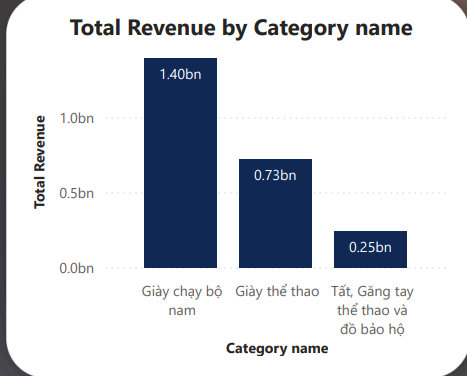
\includegraphics[width=0.72\textwidth]{images/1.1.png}
    \caption{Total revenue by category name}
\end{figure}

\begin{itemize}[leftmargin=*, label=\textbullet]
    \item \textbf{Mark:} Vertical bars.
    \item \textbf{Channel:} Bar height encodes total revenue as a quantitative measure, the X-axis position encodes category name as a categorical field, and text labels on bars reinforce exact values.
    \item \textbf{Rationale:} This chart was chosen because Objective 1.1 asks which categories contribute the most total revenue. A column chart answers that objective clearly by placing all categories on a common baseline, allowing direct comparison of revenue magnitude across groups.
    \item \textbf{Insight:} Revenue is clearly concentrated in a small number of categories. \textit{Giay chay bo nam} leads with about \textbf{1.40 billion VND}, followed by \textit{Giay the thao} at \textbf{0.73 billion VND}, while the third category contributes much less at about \textbf{0.25 billion VND}. This indicates that short-term sales performance is driven primarily by a narrow set of core categories rather than by the full catalog evenly.
\end{itemize}

\subsubsection{Objective 1.2: Category Revenue Stability and Volatility (Horizontal Bar Charts)}
\begin{figure}[H]
    \centering
    \begin{subfigure}[t]{0.48\textwidth}
        \centering
        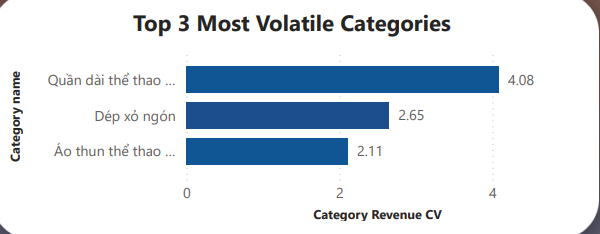
\includegraphics[width=\linewidth]{images/1.2 (1).png}
        \caption{Top 3 most volatile categories}
    \end{subfigure}
    \hfill
    \begin{subfigure}[t]{0.48\textwidth}
        \centering
        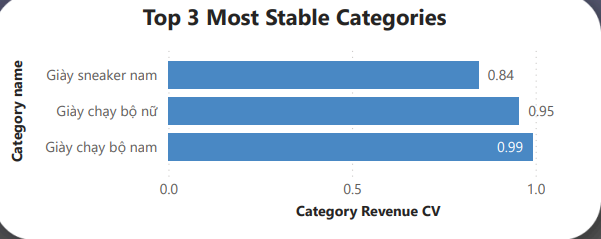
\includegraphics[width=\linewidth]{images/1.2 (2).png}
        \caption{Top 3 most stable categories}
    \end{subfigure}
    \caption{Category revenue CV comparison}
\end{figure}

\begin{itemize}[leftmargin=*, label=\textbullet]
    \item \textbf{Mark:} Horizontal bars.
    \item \textbf{Channel:} Bar length encodes \texttt{Category Revenue CV} quantitatively, the Y-axis position encodes category names categorically, and value labels show the relative degree of volatility or stability.
    \item \textbf{Rationale:} These charts were chosen because Objective 1.2 asks our group to identify and compare the most volatile and most stable categories. Horizontal bar charts answer that ranking task well by making coefficient-of-variation values easy to order, compare, and interpret side by side.
    \item \textbf{Insight:} The volatility pattern is uneven. The most volatile category reaches a CV of about \textbf{4.08}, far above the others, while the stable categories remain below \textbf{1.00}. In particular, \textit{Giay sneaker nam}, \textit{Giay chay bo nu}, and \textit{Giay chay bo nam} show relatively consistent performance, whereas categories such as long sports pants and flip-flops depend more heavily on short-lived revenue spikes.
\end{itemize}

\subsection{Theme 2: Finance Structure}

\subsubsection{Objective 2.1: Price Distribution by Price Band (Pie Chart)}
\begin{figure}[H]
    \centering
    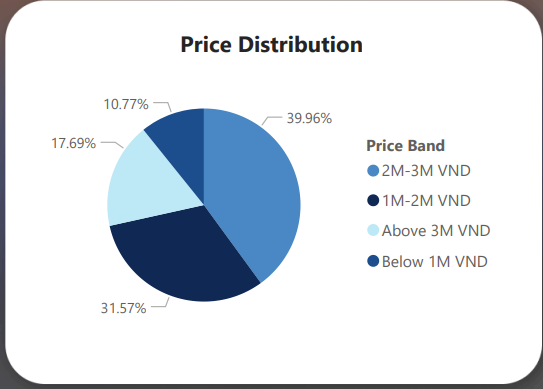
\includegraphics[width=0.72\textwidth]{images/2.1.png}
    \caption{Revenue distribution by price band}
\end{figure}

\begin{itemize}[leftmargin=*, label=\textbullet]
    \item \textbf{Mark:} Pie slices.
    \item \textbf{Channel:} Slice angle and area encode revenue share quantitatively, while color distinguishes the four categorical price bands.
    \item \textbf{Rationale:} This chart was chosen because Objective 2.1 focuses on part-to-whole comparison across a small number of price bands. A pie chart directly answers that objective by showing how total revenue is divided among the price groups and by making the dominant price band immediately visible.
    \item \textbf{Insight:} The portfolio's financial center lies in the middle price range. The \textbf{2M--3M VND} band contributes the largest share at about \textbf{39.96\%}, followed by the \textbf{1M--2M VND} band at \textbf{31.57\%}. The \textbf{Above 3M VND} and \textbf{Below 1M VND} groups contribute much smaller shares, so overall revenue is driven mainly by mid-priced products rather than extreme price segments.
\end{itemize}

\subsubsection{Objective 2.2: Top Trending Daily Revenue Pattern (Line Chart)}
\begin{figure}[H]
    \centering
    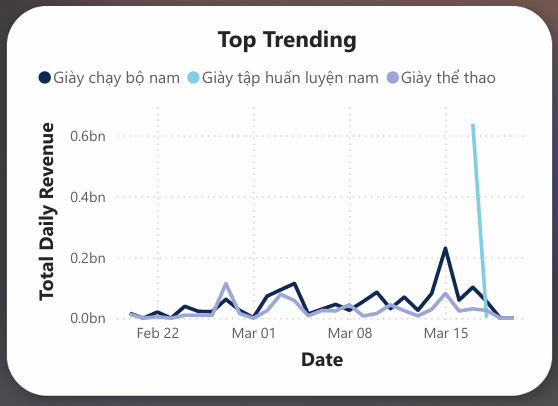
\includegraphics[width=0.78\textwidth]{images/2.2.png}
    \caption{Top trending categories by daily revenue}
\end{figure}

\begin{itemize}[leftmargin=*, label=\textbullet]
    \item \textbf{Mark:} Lines.
    \item \textbf{Channel:} Horizontal position encodes date, vertical position encodes total daily revenue, and color differentiates the leading categories shown in the chart.
    \item \textbf{Rationale:} This chart was chosen because Objective 2.2 asks whether revenue behavior is spread across time or concentrated on a small number of dates. A line chart answers that objective effectively by showing daily movement, sudden spikes, and differences in timing across the leading categories.
    \item \textbf{Insight:} Revenue movement is not evenly distributed across the period. Most dates remain at relatively low levels, but there are clear spikes in mid-March, especially for \textit{Giay tap huan luyen nam}, which rises sharply above the other categories. This suggests that page-level financial performance is shaped by a small number of high-impact dates rather than by smooth daily accumulation.
\end{itemize}

\subsection{Theme 3: Product Influence Analysis}

\subsubsection[Objective 3.1: Top Products by Average Unit Sold (Horizontal Bar Chart)]{Objective 3.1: Top Products by Average Unit Sold\texorpdfstring{\\}{ }(Horizontal Bar Chart)}
\begin{figure}[H]
    \centering
    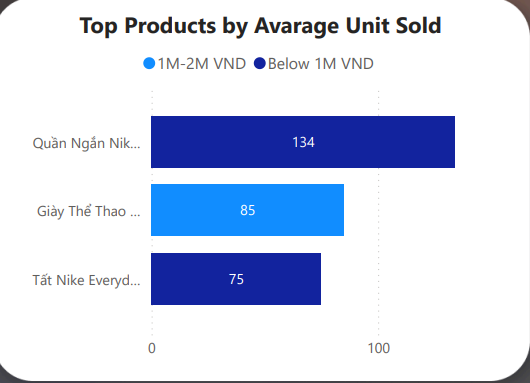
\includegraphics[width=0.72\textwidth]{images/3.1.png}
    \caption{Top products by average unit sold}
\end{figure}

\begin{itemize}[leftmargin=*, label=\textbullet]
    \item \textbf{Mark:} Horizontal bars.
    \item \textbf{Channel:} Bar length represents \texttt{Avg Daily Units Sold}, Y-axis position represents product identity, and color differentiates the associated price-band grouping shown in the legend.
    \item \textbf{Rationale:} This chart was chosen because Objective 3.1 asks which products lead unit performance. A horizontal bar chart answers that objective clearly by ranking products from strongest to weakest while also giving enough space for long product labels.
    \item \textbf{Insight:} Product influence is concentrated, but not fully monopolized by a single item. The leading product reaches about \textbf{134} average units sold, clearly ahead of the second product at \textbf{85} and the third at \textbf{75}. This shows that a small set of standout items plays an important role in unit performance, although there is still a noticeable spread across multiple top products.
\end{itemize}

\subsubsection{Objective 3.2: Top Product Unit Trend (Line Chart)}
\begin{figure}[H]
    \centering
    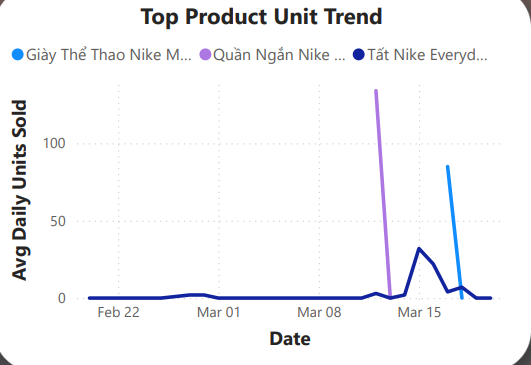
\includegraphics[width=0.72\textwidth]{images/3.2.png}
    \caption{Top product unit trend over time}
\end{figure}

\begin{itemize}[leftmargin=*, label=\textbullet]
    \item \textbf{Mark:} Lines.
    \item \textbf{Channel:} The X-axis represents date, the Y-axis represents \texttt{Avg Daily Units Sold}, and color separates the tracked top products.
    \item \textbf{Rationale:} This chart was chosen because Objective 3.2 asks whether top-product performance is stable over time or driven by a few spike dates. A line chart answers that objective better than a ranking chart because it preserves the time sequence and highlights sudden increases in units sold.
    \item \textbf{Insight:} The strongest products do not perform uniformly across the full period. Instead, the chart shows several sharp spikes in mid-March, including one product peaking above \textbf{130} units and another later peak near \textbf{85} units. This indicates moderate concentration risk: short-term product influence depends partly on a few strong surge dates rather than on perfectly stable demand.
\end{itemize}

\subsection{Theme 4: Customer Ratings and Review Signals}

\subsubsection[Objective 4.1: Monthly Rating and Review Trends (Dual-Axis Line Chart)]{Objective 4.1: Monthly Rating and Review Trends\texorpdfstring{\\}{ }(Dual-Axis Line Chart)}
\begin{figure}[H]
    \centering
    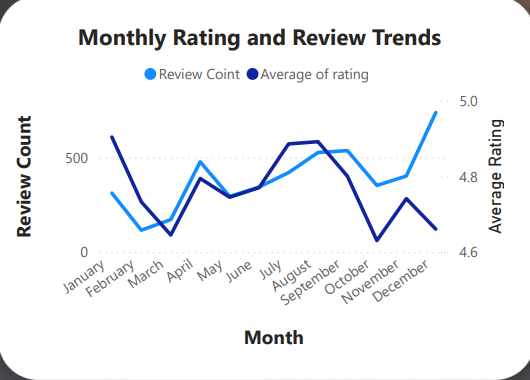
\includegraphics[width=0.72\textwidth]{images/4.1.png}
    \caption{Monthly rating and review trends}
\end{figure}

\begin{itemize}[leftmargin=*, label=\textbullet]
    \item \textbf{Mark:} Two lines on a dual-axis chart.
    \item \textbf{Channel:} The X-axis encodes month, the left Y-axis encodes review count, the right Y-axis encodes average rating, and color distinguishes the two measures.
    \item \textbf{Rationale:} This chart was chosen because Objective 4.1 asks our group to compare two monthly signals at the same time: review count and average rating. A dual-axis line chart answers that objective well by placing both measures on the same timeline while keeping their different numeric scales readable.
    \item \textbf{Insight:} Customer sentiment remains generally high, with the rating line staying in the upper 4.6 to 4.9 range, while review volume varies more noticeably by month. Review activity rises strongly in April and again toward December, whereas average rating dips more clearly around March and November. This means customer attention fluctuates more than customer satisfaction does.
\end{itemize}

\subsubsection[Objective 4.2: Monthly Comment Trends for Top Products (Line Chart)]{Objective 4.2: Monthly Comment Trends for Top Products\texorpdfstring{\\}{ }(Line Chart)}
\begin{figure}[H]
    \centering
    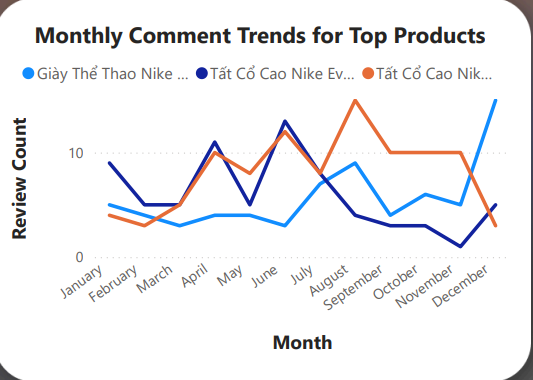
\includegraphics[width=0.72\textwidth]{images/4.2.png}
    \caption{Monthly comment trends for top products}
\end{figure}

\begin{itemize}[leftmargin=*, label=\textbullet]
    \item \textbf{Mark:} Lines.
    \item \textbf{Channel:} Horizontal position represents month, vertical position represents review count, and color differentiates the most-discussed products.
    \item \textbf{Rationale:} This chart was chosen because Objective 4.2 asks which products receive the most comments across months and whether that attention stays concentrated. A multi-line chart answers that objective clearly by showing changes in monthly leadership, persistence, and spikes for each tracked product.
    \item \textbf{Insight:} Customer discussion is not dominated by one product throughout the year. Different products lead in different months: one line peaks strongly in August, another becomes more prominent around June, and another jumps highest in December. This suggests that review attention rotates across products rather than remaining permanently concentrated in a single item.
\end{itemize}

\subsection{Theme 5: Machine Learning Insights (Clustering)}

\subsubsection{Objective 5.1: Clustering Quality and Segment Identification (Bar Chart and Scatter Plot)}
\begin{figure}[H]
    \centering
    \begin{subfigure}[t]{0.48\textwidth}
        \centering
        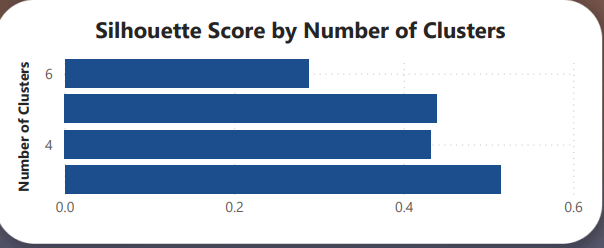
\includegraphics[width=\linewidth]{images/5.1.png}
        \caption{Silhouette score by number of clusters}
    \end{subfigure}
    \hfill
    \begin{subfigure}[t]{0.48\textwidth}
        \centering
        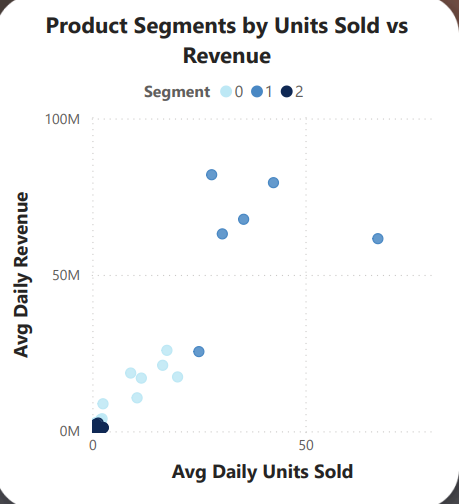
\includegraphics[width=\linewidth]{images/5.2 (1).png}
        \caption{Product segments by units sold vs revenue}
    \end{subfigure}
    \caption{Clustering quality and segment identification}
\end{figure}

\begin{itemize}[leftmargin=*, label=\textbullet]
    \item \textbf{Mark:} Horizontal bars in the silhouette chart and points in the scatter plot.
    \item \textbf{Channel:} In the first visual, bar length encodes silhouette score and Y-axis position encodes the candidate number of clusters. In the second visual, X-axis position encodes \texttt{Avg Daily Units Sold}, Y-axis position encodes \texttt{Avg Daily Revenue}, and color encodes cluster membership.
    \item \textbf{Rationale:} These charts were chosen because Objective 5.1 has two linked tasks: selecting a reasonable clustering solution and checking whether the resulting segments are visibly distinct. The silhouette-score bar chart answers the model-selection part, while the scatter plot answers the segment-identification part by showing whether products separate into different performance regions.
    \item \textbf{Insight:} The \textbf{3-cluster} solution appears to be the strongest because it has the highest silhouette score, around \textbf{0.53}, while the alternatives with 4, 5, and 6 clusters perform worse. The scatter plot also shows meaningful separation between low-performing products near the origin, mainstream products in the middle range, and a smaller high-performing group with much larger units sold and revenue values.
\end{itemize}

\subsubsection{Objective 5.2: Cluster Revenue Contribution Interpretation (Scatter Plot and Pie Chart)}
\begin{figure}[H]
    \centering
    \begin{subfigure}[t]{0.48\textwidth}
        \centering
        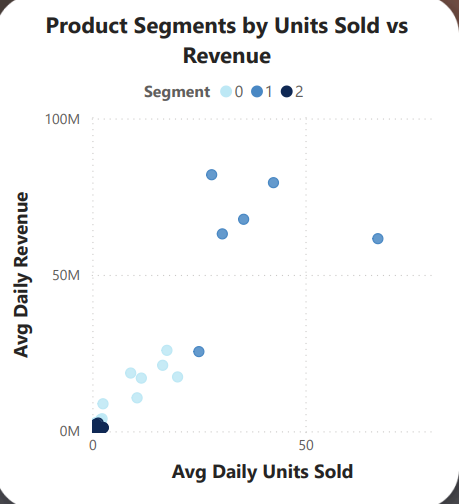
\includegraphics[width=\linewidth]{images/5.2 (1).png}
        \caption{Product segments by units sold vs revenue}
    \end{subfigure}
    \hfill
    \begin{subfigure}[t]{0.48\textwidth}
        \centering
        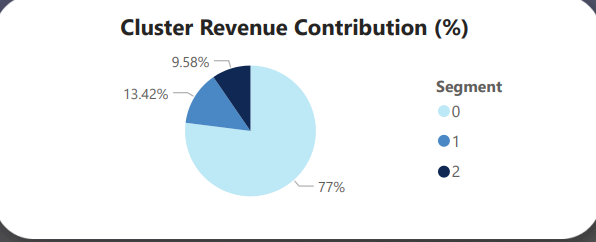
\includegraphics[width=\linewidth]{images/5.2 (2).png}
        \caption{Cluster revenue contribution}
    \end{subfigure}
    \caption{Cluster contribution to overall sales performance}
\end{figure}

\begin{itemize}[leftmargin=*, label=\textbullet]
    \item \textbf{Mark:} Points in the scatter plot and pie slices in the contribution chart.
    \item \textbf{Channel:} The scatter plot uses spatial position to compare performance by units sold and daily revenue, while the pie chart uses slice area and color to show each segment's share of total revenue.
    \item \textbf{Rationale:} These charts were chosen because Objective 5.2 asks not only how clusters differ, but also how much each cluster contributes to overall sales performance. The scatter plot explains the behavioral profile of each segment, while the pie chart directly answers the contribution question by showing revenue share across clusters.
    \item \textbf{Insight:} Segment \textbf{0} contributes the largest share of total revenue at about \textbf{77\%}, so the mainstream product group remains the main commercial base of the portfolio. The remaining segments contribute about \textbf{13.42\%} and \textbf{9.58\%}, which shows that smaller groups still matter but play more specialized roles. Combined with the scatter plot, this indicates that overall revenue is dominated by the broad central segment rather than by the extreme high-performing or low-performing groups alone.
\end{itemize}

\subsection{Overall Summary of Findings}

The objective-based visual analysis supports the group's common analytical problem in a coherent way. Category revenue is concentrated in a few strong groups, the portfolio's financial center lies in the 1M--3M VND range, and product influence is shaped by several standout items with visible mid-March spikes. Customer review volume changes more strongly than average rating, while the clustering layer shows that the catalog can be meaningfully separated into segments with different performance profiles and different revenue contributions.

Overall, the report now aligns the analysis narrative directly with the dashboard evidence used in the final submission. This makes Section 3 more consistent with the actual visuals, easier to defend in presentation, and more clearly connected to the measurable objectives introduced in Section 1.



\FloatBarrier

\newpage


% === file này không sửa gì vào nha, thêm ref ở file ref.bib

\cleardoublepage
\phantomsection
\addcontentsline{toc}{section}{References}
\nocite{*}
\bibliographystyle{unsrt}
\bibliography{ref}



\end{document}


